\section{Peripherals}
\label{sec:periphs}

attached to the data bus is shown in Figure~\ref{fig:periphs}.

\begin{figure}[!htbp]
    \centerline{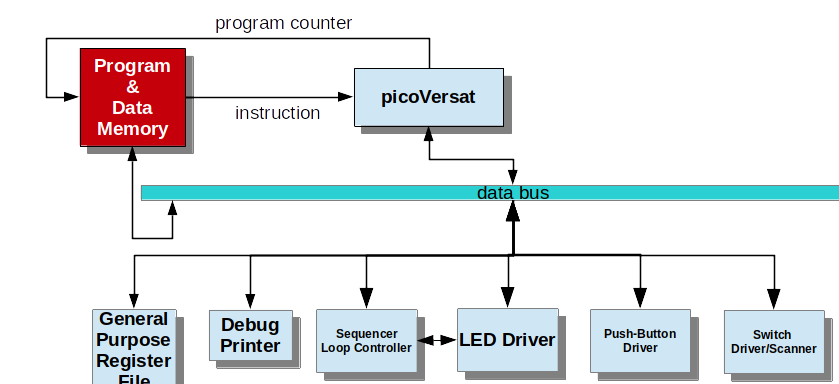
\includegraphics[width=\textwidth]{periphs.png}}
    \vspace{0cm}\caption{PicoVersat SoC with two peripherals}
    \label{fig:periphs}
\end{figure}

Refer to the memory map in section~\ref{sec:mem_map} to check the base addresses
of the peripherals.

\subsection{General Purpose Register File}

This peripheral contains a 16x32bit register file that can be used by user
programs. 

\subsection{Debug Printer}

This peripheral can be used by user programs to print characters, mainly for
debug purposes.

\subsection{LED Driver}

Led driver.

\subsection{Switch Driver/Scanner}

Switch Driver.

\subsection{Push-Button Driver}

Push-Button Driver.

\subsection{Frequency Generator}

Frequency Generator.

